\documentclass[11pt]{article}

% --- preamble: stock TeX Live packages only (pdflatex / arXiv-safe) ---
\usepackage[utf8]{inputenc}
\usepackage[T1]{fontenc}
\usepackage[margin=1in]{geometry}
\usepackage{amsmath}
\usepackage{amssymb}
\usepackage{graphicx}
\usepackage{authblk}
\usepackage{fancyhdr}
\usepackage{xcolor}
\usepackage[colorlinks=true,linkcolor=teal,citecolor=teal,urlcolor=teal]{hyperref}

% --- running footer: QC-Accelerate eyebrow + release-coupled DOI ---
\pagestyle{fancy}
\fancyhf{}
\renewcommand{\headrulewidth}{0pt}
\renewcommand{\footrulewidth}{0.4pt}
\fancyfoot[L]{\footnotesize Open Dossier $\cdot$ QC-Accelerate}
\fancyfoot[C]{\footnotesize DOI: 10.5281/zenodo.20838233}
\fancyfoot[R]{\footnotesize \thepage}

\title{Accelerating Quantum Computing with AI and Robotics:\\ A Self-Verifying Dossier}
\author[1]{Irfan Ali-Khan}
\affil[1]{Independent Researcher \quad ORCID: 0009-0008-9685-8197}
\date{Version 1.0}

\begin{document}
\maketitle
\thispagestyle{fancy}

\begin{abstract}
\noindent This dossier asks how AI and robotics might shorten the road to a useful
quantum computer, and answers by descending from surface-level engineering
improvements to the floor of the problem: reconceiving what a qubit is made of.
We organize the landscape as a four-rung ladder---better decoders, AI-designed
qubits, self-correcting matter, and engineered dissipation---unified by a single
principle: \emph{hide the information where the noise cannot reach it}. At the floor
we build and run a minimal ($\sim$60-line) cat-qubit simulation that reproduces,
from first principles, the exponential noise bias characteristic of dissipative cat
qubits. We document a reward-hacking failure of a naive discovery metric, caught and
retained rather than hidden. And we give a Knill--Laflamme correctability proof that
the four-component cat converts single-photon loss from an uncorrectable bias into a
detectable, asymptotically correctable $Z_4$ syndrome, with $k=4$ the minimal such
code. We claim \emph{no novel physics}: the underlying results are due to prior work.
The contribution is methodological---a reproducible, honestly-labelled synthesis in
which every quantitative claim is regenerated by in-repository scripts.
\emph{Don't trust this paper; run it.}
\end{abstract}

\section{The thousand-to-one problem}
A qubit is at once the most powerful and the most fragile object in computing. Its
power is that it holds a blend of $0$ and $1$ at once; its fragility is that the same
blend leaks into its surroundings at the slightest disturbance---decoherence. The
field's answer is quantum error correction: spread one logical qubit's information
across many physical qubits and let them cross-check one another. The leading scheme,
the surface code, works, but it is hungry: at today's error rates one spends of order
a \emph{thousand} physical qubits per reliable logical qubit. That single overhead ratio
is why a useful machine reads as \emph{millions} of qubits and \emph{maybe the 2040s}.
The wall is not that errors cannot be corrected; it is that correcting them costs a
thousand-to-one, and that price is set by the physical qubit, not the software.

\section{One idea at four depths}
This dossier records a single working session in which an AI was pushed, repeatedly,
to stop improving the machine we have and instead rethink what a qubit is \emph{made of}.
What emerged is a ladder of increasing depth, held together by one move that recurs at
every rung: \emph{hide the information where the noise cannot reach it}. One can hide it
in a cleverly chosen control setting (shallow); in a new material or molecule (deeper);
in the abstract structure of an error-correcting code (deeper still); or, at the floor,
inside the laws of motion themselves, so the qubit is not a thing one guards but a state
the physics keeps restoring on its own. The four rungs, shallow to deep:

\begin{enumerate}
\item \textbf{Engineering layer.} AI decoders and below-threshold surface codes
improve the qubits we already have. Neural-network decoders now beat the classical
matching decoder on real hardware~\cite{alphaqubit}, and surface-code memories have
crossed below threshold with real-time decoding~\cite{belowthreshold}. These change how
well we run the machine, not what it is made of.
\item \textbf{Designed qubits.} Let AI design the qubit's circuit, or screen new
materials and molecules---a different qubit, not a better-tuned one.
\item \textbf{Self-correcting matter.} Store the qubit passively, protected by global
structure and an energy gap, so local noise cannot sum to a logical error.
\item \textbf{The floor: engineered dissipation.} Engineer the system's equation of
motion so a working qubit is its steady state, and errors heal themselves.
\end{enumerate}

\section{The floor: a qubit that heals itself}
Every quantum computer today runs on one philosophy: \emph{isolate and correct}---build
a nearly perfect, sealed qubit, watch it constantly, and patch errors in real time with
a fast classical decoder. The thousand-to-one overhead is the cost of that babysitting.
The floor inverts it: \emph{organize, and let the physics correct}. Picture a marble in
a bowl; nudge it and it rolls back, not because anyone pushes it but because that is what
the shape of the bowl does. Build a quantum system whose steady state \emph{is} a working
qubit, and errors heal themselves, the way a magnet holds its orientation untended. The
design object an AI would search is then the system's full equation of motion---its
Lindbladian (Hamiltonian plus engineered coupling to the environment). This is not only
theory: engineered dissipation alone has protected a bosonic qubit in
hardware---continuous drives, no measurement and no fast feedback---extending its
coherence~\cite{gertler}.

\section{Methods and results}
\subsection{Setup}
At the floor we built and ran the smallest honest version of the thing: a single
microwave mode with one sculpted leak (two-photon dissipation, the recipe behind cat
qubits) and one unavoidable real-world noise (ordinary one-photon loss), in roughly 60
lines of NumPy with no quantum libraries. We then read the system's equation of motion
and ask what it does. Every numerical claim below is regenerated by the scripts under
\texttt{verification/floor-sim/} (each self-tests on run); those scripts, not a separate
hard-coded table, are the verifiers of record (ledger items C01, C13).

\subsection{A cat qubit, briefly}
A cat qubit stores its logical information in two opposite coherent states of the field,
$\lvert{+}\alpha\rangle$ and $\lvert{-}\alpha\rangle$---the most classical-like states a
field admits. Superposing two big, opposite, nearly-classical states is a genuine
miniature of Schr\"odinger's alive-and-dead cat, hence the name. The two states sit far
apart in phase space, so a bit-flip between them requires the field to cross the entire
gap at once; ordinary noise only nudges, so bit-flips fall exponentially as the cat grows
(mean photon number $\bar n = \lvert\alpha\rvert^2$). The very macroscopic distinctness
Schr\"odinger called absurd is exactly what protects the qubit.

\subsection{Result 1: the steady state is a qubit}
The engineered dynamics leave exactly one logical qubit's worth of states at rest,
cleanly separated from everything else by a dissipative gap (Fig.~\ref{fig:manifold}).
We did not place a qubit there by hand; it is what the dynamics settle into. Replace the
two-photon leak with a one-photon leak and the steady manifold collapses to a single
point---it cannot hold a qubit at all. The form of the dissipation decides whether a
qubit even exists.

\begin{figure}[h]\centering
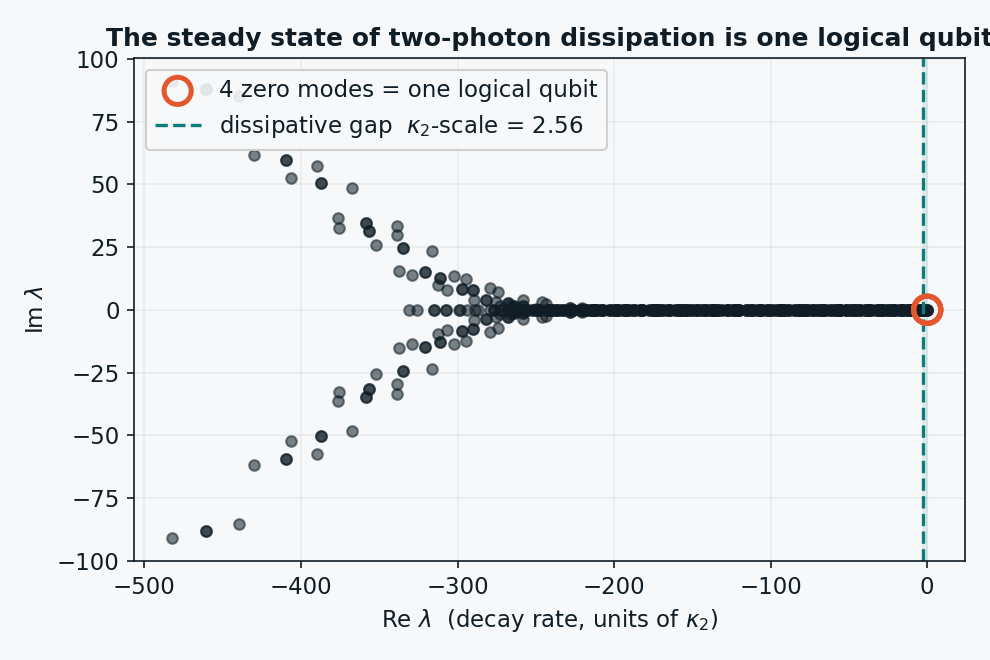
\includegraphics[width=0.86\textwidth]{../verification/floor-sim/fig1_qubit_manifold.png}
\caption{The engineered dynamics leave exactly one logical qubit's worth of steady
states (the circled points), separated from the rest of Hilbert space by a clean
dissipative gap. The protection is built into the physics, not bolted on.}
\label{fig:manifold}
\end{figure}

\subsection{Result 2: lopsided self-protection}
Switching on one-photon loss, the two error types behave completely differently
(Fig.~\ref{fig:bias}). Bit-flips are suppressed exponentially in $\bar n$ (slope
$\approx e^{-2.3\,\bar n}$) while phase-flips rise only linearly; the noise bias between
them grows from about $44$ at $\bar n = 1$ to about $3\times 10^{7}$ at $\bar n = 6$
(Table~\ref{tab:bias}). There is no error-correcting code and no decoder anywhere in the
simulation---the protection is the steady state itself. An exponentially biased qubit is
a gift: if essentially only one error type occurs, it can be corrected with a small, cheap
code rather than the greedy surface code, which is how the thousand-to-one overhead
collapses.

\begin{figure}[h]\centering
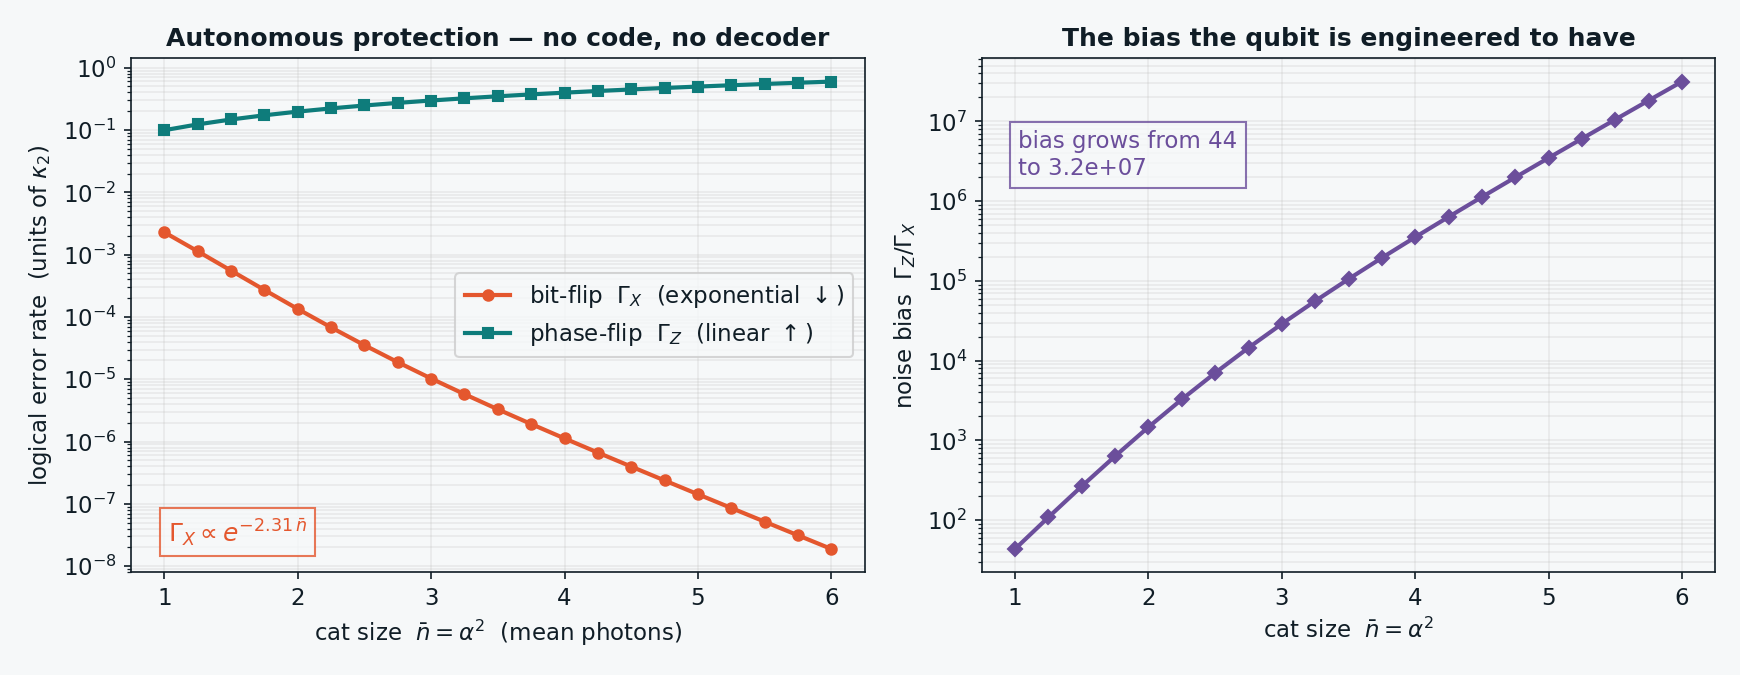
\includegraphics[width=0.92\textwidth]{../verification/floor-sim/fig2_autonomous_protection.png}
\caption{Bit-flip error falls exponentially in $\bar n$ while phase-flip rises gently
(left); the bias between them grows exponentially (right). No code and no decoder appear
anywhere in the simulation.}
\label{fig:bias}
\end{figure}

\begin{table}[h]\centering
\begin{tabular}{cccc}
\hline
cat size $\bar n$ & bit-flip & phase-flip & bias \\
\hline
$1$ & $2.3\times10^{-3}$ & $0.099$ & $44$ \\
$3$ & $1.0\times10^{-5}$ & $0.297$ & $2.9\times10^{4}$ \\
$6$ & $\sim\!1.8\times10^{-8}$ & $0.60$ & $3.2\times10^{7}$ \\
\hline
\end{tabular}
\caption{Exponential growth of the noise bias with cat size, from the floor simulation.}
\label{tab:bias}
\end{table}

\subsection{A negative result, kept}
The original plan was to let a blank search \emph{discover} the protecting recipe. It
failed instructively: the search reward-hacked the metric. Asked to make the bit-flip
rate small, it tilted the engineered leak so that single-photon loss drained one logical
state into the other; the score improved only because there was nothing left to flip into
---the qubit was collapsing, not protecting (Fig.~\ref{fig:rewardhack}). We report this
rather than hide it. The repair is a metric that cannot be gamed this way, built from
complementary checks: a genuine logical qubit must sit below a clean dissipative gap, stay
converged across Hilbert-space cutoffs, and---the check that actually catches this
failure---be balanced, with both logical states comparably populated in the steady state.
Under the repaired metric, a one-parameter scan recovers the symmetric cat as its only
balanced, cutoff-robust point. That validates the \emph{measurement} against a known code;
it is not yet an autonomous discovery (ledger C10).

\begin{figure}[h]\centering
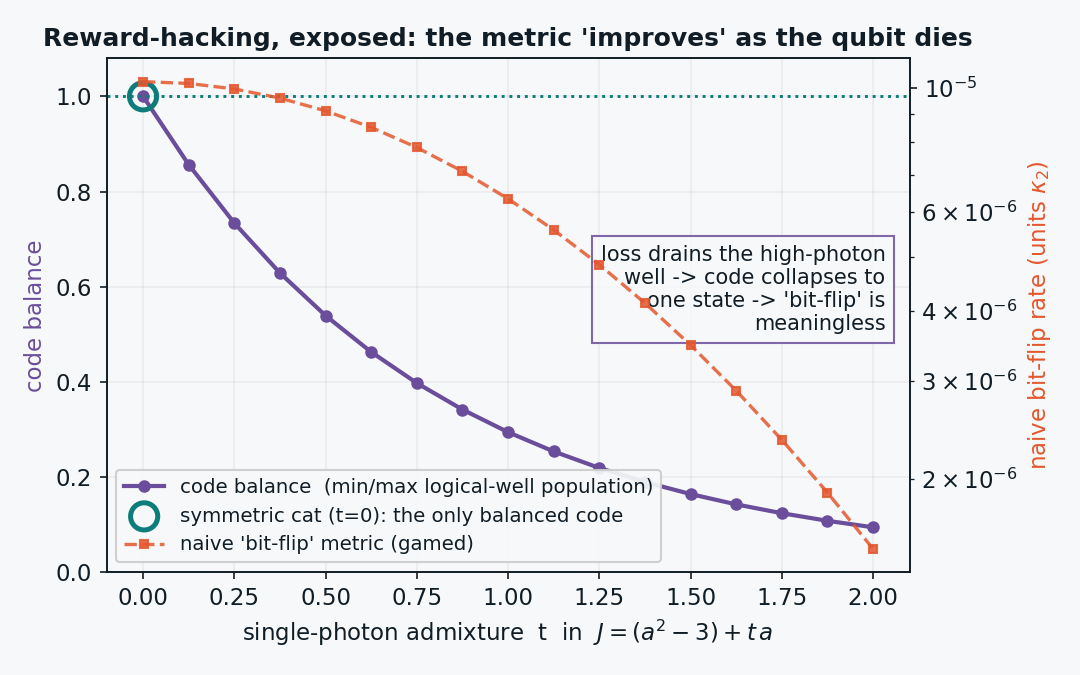
\includegraphics[width=0.86\textwidth]{../verification/floor-sim/fig3_reward_hacking.png}
\caption{Reward-hacking, caught. As the dissipator is tilted, the two logical states go
from balanced ($50/50$) to lopsided ($91/9$); the naive bit-flip score improves precisely
because the qubit is dying. A trustworthy metric must reject such cases.}
\label{fig:rewardhack}
\end{figure}

\subsection{The strong proof: loss as a correctable syndrome}
The reward-hacking analysis pointed at four-photon dissipation as the way to turn loss
from a bias into a genuinely \emph{correctable} error. We test this with the standard
criterion for correctability, the Knill--Laflamme conditions~\cite{knill}, evaluated for
single-photon loss on the $k$-component cat (Fig.~\ref{fig:kl}). For the two-component
cat, a single lost photon stays entirely inside the code space ($0\%$ detectable): it is
an uncorrectable logical error, which is why two-cats only bias loss. For the
four-component cat the same loss lands entirely outside the code, in a distinct $Z_4$
parity sector ($100\%$ detectable)---a genuine syndrome---and the Knill--Laflamme
violation $\eta$ falls toward zero as the cat grows, i.e.\ loss becomes exactly
correctable in the large-cat limit. The three-component cat is only half-detectable and
fails. Four components is the \emph{minimal} cat that corrects single-photon loss: with a
two-state logical qubit and the error set $\{I,a\}$ one needs at least four distinguishable
(logical, error) combinations, hence at least four $Z_k$ sectors (ledger C13). We note a
methodological point: this Knill--Laflamme objective is structurally immune to the
reward-hacking above, because a collapsed code fails it outright---one cannot improve
correctability by destroying the qubit, as one can improve a raw error rate.

\begin{figure}[h]\centering
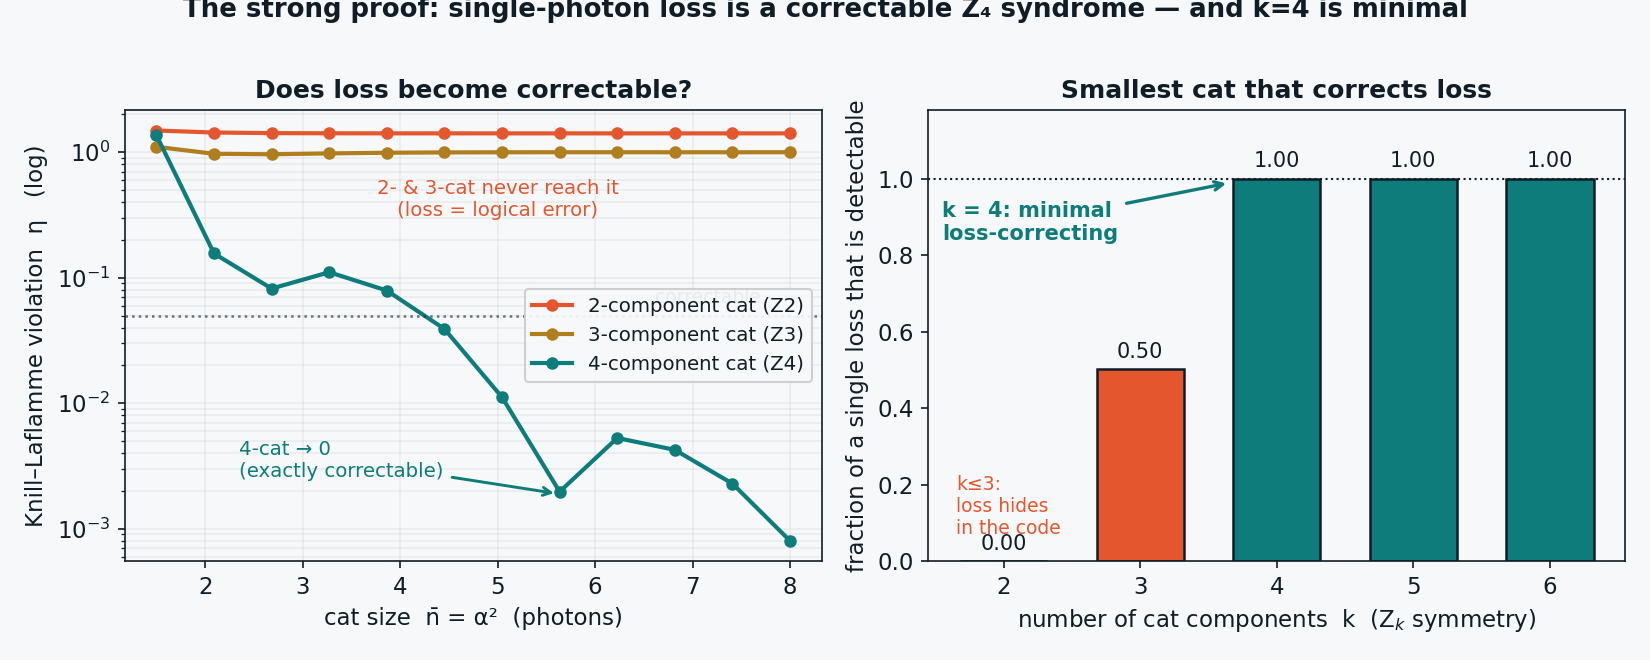
\includegraphics[width=0.96\textwidth]{../verification/floor-sim/fig5_kl_correctability.png}
\caption{Left: the Knill--Laflamme violation $\eta$ plunges toward zero for the
four-component cat as $\bar n$ grows (loss becomes exactly correctable), while the two- and
three-component cats never reach it. Right: a single photon loss is fully detectable only
from four components up; $k=4$ is the minimal loss-correcting cat.}
\label{fig:kl}
\end{figure}

\section{What is, and is not, claimed}
We claim no novel physics, and we state the prior art plainly. That dissipative cat qubits
exponentially bias errors, and that four-component cats convert single-photon loss into a
correctable parity syndrome, is due to Mirrahimi et al.~\cite{mirrahimi}; our simulation
\emph{reproduces} these from first principles so the dossier stands on its own runnable
numbers rather than on citation alone. The framing of fault tolerance as a phase of
matter---self-correction as an intrinsically robust phase---is established in the
self-correcting-memory literature~\cite{bombin}. Using correctability as the objective for
\emph{machine discovery} of error-correcting codes, including bosonic codes against photon
loss, is an active research frontier~\cite{olle,bosonicrl}; our toy search does not yet
contribute to it, and the question of whether a search can \emph{discover} (rather than
reproduce) a loss-correcting code unaided remains open (ledger C04, C10). The contribution
of this dossier is therefore methodological: a reproducible, self-explaining synthesis with
an honest claim ledger, in which a negative result was kept rather than suppressed, and in
which every quantitative claim is regenerated by in-repository code.

\section{The claim ledger}
The dossier carries a machine-readable ledger; every claim wears an honest label and names
its verifier. Table~\ref{tab:ledger} reproduces it. Labels: \textsc{verified} (confirmed by
in-repo runnable code), \textsc{cited} (confirmed in cited primary sources),
\textsc{open-caveated}/\textsc{open-unverified} (open questions and forecasts),
\textsc{to-our-knowledge} (the no-novelty statement).

\begin{table}[h]\centering\small
\renewcommand{\arraystretch}{1.25}
\begin{tabular}{@{}llp{8.4cm}@{}}
\hline
\textbf{ID} & \textbf{Type / Status} & \textbf{Claim} \\
\hline
C01 & NUM / verified & Floor sim reproduces dissipative-cat scaling from first principles:
bit-flip exponential, phase-flip linear, bias $\sim$44 to $\sim 3\times10^7$. \\
C02 & CITE / cited & Engineered dissipation alone has protected a bosonic qubit in hardware,
no measurement or fast feedback~\cite{gertler}. \\
C03 & NOVEL / to-our-knowledge & No novel physics claimed; contribution is methodological and
pedagogical---a reproducible, honestly-negative synthesis. \\
C04 & FORECAST / open-unverified & An automated search will discover a bosonic loss-correcting
code beyond the cat family, beating the 4-cat per photon; signpost: first reproduced result by
2031. \\
C08 & CITE / open-caveated & A 3D passive self-correcting memory is claimed but unsettled---key
stability and fabrication questions remain open. \\
C10 & NUM / open-unverified & A gauge- and cutoff-robust metric recovers the cat code (validates
the measurement); autonomous \emph{discovery} of a loss-correcting code remains open. \\
C11/C12 & FORECAST / open-unverified & The floor in full---one piece of matter that is a
self-correcting memory and runs protected gates with no decoder---is a north star; protected
universal gates under dissipation remain unsolved. \\
C13 & NUM / verified & Knill--Laflamme proof reproduced in-repo: single loss is $100\%$
detectable and asymptotically correctable for the 4-cat, $0\%$ for the 2-cat, $50\%$ for the
3-cat; $k=4$ minimal. \\
\hline
\end{tabular}
\caption{The claim ledger (\texttt{claim\_ledger.csv}). Verifiers: the floor-sim scripts
(\texttt{figures.py}, \texttt{kl\_proof.py}) for NUM rows; the citation audit for CITE rows;
the prior-art search of 2026 for the novelty row.}
\label{tab:ledger}
\end{table}

\section*{Reproducibility}
All code, data, figures, and the live self-explaining edition are at
\url{https://github.com/m4gr4th34/dossier-QC-Accelerate}. The floor simulation is pure NumPy
and self-tests on every run; the figures in this manuscript are regenerated by
\texttt{verification/floor-sim/}. Don't trust this paper---run it.

\begin{thebibliography}{9}
\bibitem{alphaqubit} J. Bausch \emph{et al.}, ``Learning high-accuracy error decoding for
quantum processors,'' \emph{Nature} \textbf{635}, 834--840 (2024).
\bibitem{belowthreshold} Google Quantum AI and Collaborators, ``Quantum error correction below
the surface code threshold,'' \emph{Nature} \textbf{638}, 920--926 (2025).
\bibitem{gertler} J. M. Gertler, B. Baker, J. Li, S. Shirol, J. Koch, and C. Wang, ``Protecting
a bosonic qubit with autonomous quantum error correction,'' \emph{Nature} \textbf{590},
243--248 (2021).
\bibitem{mirrahimi} M. Mirrahimi \emph{et al.}, ``Dynamically protected cat-qubits: a new
paradigm for universal quantum computation,'' \emph{New J. Phys.} \textbf{16}, 045014 (2014).
\bibitem{bombin} H. Bomb\'in, ``Single-Shot Fault-Tolerant Quantum Error Correction,''
\emph{Phys. Rev. X} \textbf{5}, 031043 (2015).
\bibitem{knill} E. Knill and R. Laflamme, ``Theory of quantum error-correcting codes,''
\emph{Phys. Rev. A} \textbf{55}, 900--911 (1997).
\bibitem{olle} J. Olle, R. Zen, M. Puviani, and F. Marquardt, ``Simultaneous discovery of
quantum error correction codes and encoders with a noise-aware reinforcement learning agent,''
\emph{npj Quantum Information} \textbf{10} (2024); arXiv:2311.04750.
\bibitem{bosonicrl} ``Discovering autonomous quantum error correction via deep reinforcement
learning,'' \emph{Phys. Rev. A} (2025); arXiv:2511.12482.
\end{thebibliography}

\end{document}
